\documentclass[11pt]{article}

\usepackage[letterpaper]{geometry}

\usepackage[utf8]{inputenc}
\usepackage{mathpazo}
\usepackage{amsmath}
\usepackage{amsfonts}
\usepackage{physics}
\usepackage{siunitx}

\usepackage{fancyhdr}

\usepackage{graphicx}
\usepackage{float}
\usepackage{booktabs}

\usepackage[shortlabels,inline]{enumitem}

% Hyperlinks with decent looking default colors.
\usepackage{hyperref}
\usepackage{xcolor}
\hypersetup{
  colorlinks,
  linkcolor={red!50!black},
  citecolor={blue!50!black},
  urlcolor={blue!80!black}
}

% For those sexy spaced low small caps from classic-thesis!
\usepackage{microtype}
\usepackage{textcase}
\DeclareRobustCommand{\spacedlowsmallcaps}[1]{%
  \textls[80]{\scshape\MakeTextLowercase{#1}}%
}

\pagestyle{fancy} 
\fancyhead{}
\rhead{Ali Ramadhan}
\lhead{12.818: Project 3}
\chead{}
\cfoot{\thepage}

\title{\spacedlowsmallcaps{\small 12.818: Introduction to Atmospheric Data and Large-scale Dynamics}\\ \spacedlowsmallcaps{\Large Project three: Convection and atmospheric thermodynamics}}
\author{\spacedlowsmallcaps{Ali Ramadhan}}
\date{}

% \renewcommand\thesection{\Alph{section}}

\begin{document}
\maketitle

In this project we will investigate the nature of convection in the lower troposphere, which is the mechanism responsible for transporting heat from terrestrial radiation vertically upward to the upper troposphere where water vapor concentration and thus infrared absorption is much lower, allowing it to be emitted to outer space.

To carry out this investigation, we will used observed temperature profiles from radiosonde soundings to study the onset of convection in the lower atmosphere.

\section{Stability to dry processes}
Plotting the given temperature profile for standard atmospheric conditions at the mid-latitudes on a full-size ($29\times21.5$ in) skew $T$ $\log P$ graph, we can answer the given questions.
\begin{enumerate}
	\item The tropopause can be identified as the region where an abrupt change in the lapse rate occurs. By inspection, we see this happens somewhere between \SIrange{300}{200}{\hecto\Pa} with the reference temperature profile indicating that it occurs at around \SI{225}{\hecto\Pa}.
	\item We see that dry air is unstable only up to the lifted condensation level and then becomes stable, but moist air is unstable all the way up to \SI{525}{\hecto\Pa} at which point it becomes stable.
	\item The mixing ratio at \SI{1000}{\hecto\Pa} is \SI{9.5}{\g\per\kg}, and at \SI{500}{\hecto\Pa} it is just above \SI{1.5}{\g\per\kg} indicating drier conditions as expected.
	\item If the surface cools radiatively during the night, the air just needs to cool by \SI{2}{\degree C} for it to reach the same temperature as the dew point and for fog to form.
	\item If the air is heated the following day and rises adiabatically, condensation will occur above the lifted condensation level (LCL) which occurs where a lifted air parcel reaches 100\% relative humidity. For our temperature profile, this happens around \SI{950}{\hecto\Pa} (\SI{540}{\m}) where the moist adiabat from the dew point crosses the dry adiabat from the surface temperature.
	\item Condensation can continue happening until around \SI{525}{\hecto\Pa} at which point the atmosphere becomes stable and convection stops.
\end{enumerate}

Given the saturation vapor pressure $e_s$ as a function of $T$ with 4 data points, $(\SI{6.11}{\hecto\Pa}, \SI{0}{\degreeCelsius})$, $(\SI{13.0}{\hecto\Pa}, \SI{10}{\degreeCelsius})$, $(\SI{23.4}{\hecto\Pa}, \SI{20}{\degreeCelsius})$, and $(\SI{1000}{\hecto\Pa}, \SI{100}{\degreeCelsius})$, we can fit the data points to the phenomenological model $e_s(T) = Ae^{\beta T}$. Doing so provides a perfect looking fit ($R^2 = 1$) with parameter values of $A = \SI{8.419}{\hecto\Pa}$ and $\beta = \SI{0.0477}{\per\K}$ although more data would be nice to ensure that this model holds for all physically realizable atmospheric pressures and obtain a more certain fit. From this model, we can calculate the saturation specific humidity $q_\star$ at \SI{850}{\hecto\Pa} using
\begin{equation*}
  q_\star(p,T) = \frac{\epsilon e_s(T)}{p}
\end{equation*}
where $\displaystyle \epsilon = \frac{18}{29}$ is the ratio of water vapor's molecular mass to that of air. We can thus obtain $q_\star(\SI{850}{\hecto\Pa}, \SI{4}{\degreeCelsius}) = \SI{7.4}{\g/\kg}$ where we took \SI{4}{\degreeCelsius} to be the temperature at \SI{850}{\hecto\Pa} according to the skew $T$ $\log P$ diagram we were given. 

\section{Dry convection}
Inspecting the dry deserts of the United States, we notice that Arizona may be a good candidate for looking at dry convection. In particular, we see that Tucson, AZ might be a particularly good example. Figure \ref{fig:TUS0Z} shows a temperature profile for Tuczon at 0Z (16:00 MST) and \ref{fig:TUS12Z} shows a temperature profile at 12Z (04:00 MST).

\begin{figure}[h!]
  \centering
  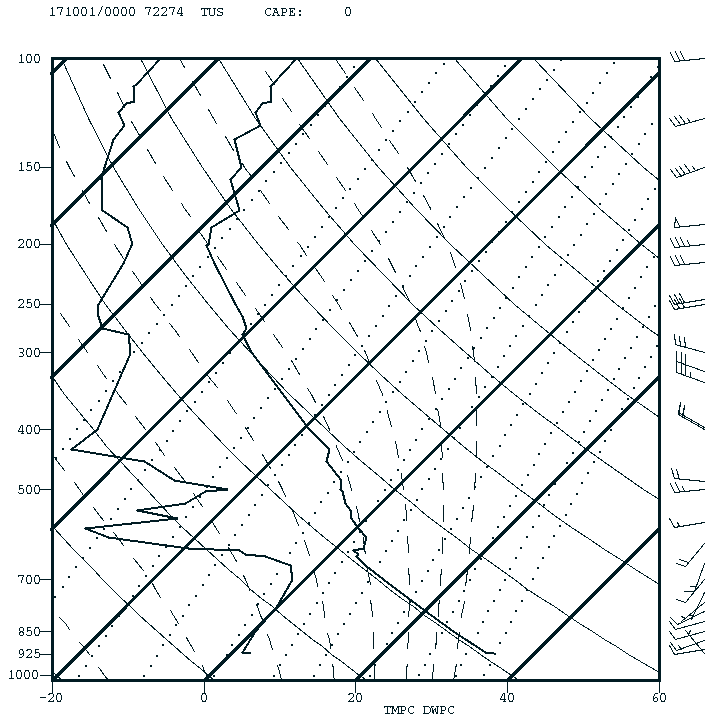
\includegraphics[width=\textwidth]{TUSTempProfile0Z.png}
  \caption{Temperature profile over Tucson, AZ on October 1, 2017 at 0Z (16:00 MST).}
  \label{fig:TUS0Z}
\end{figure}

\begin{figure}[h!]
  \centering
  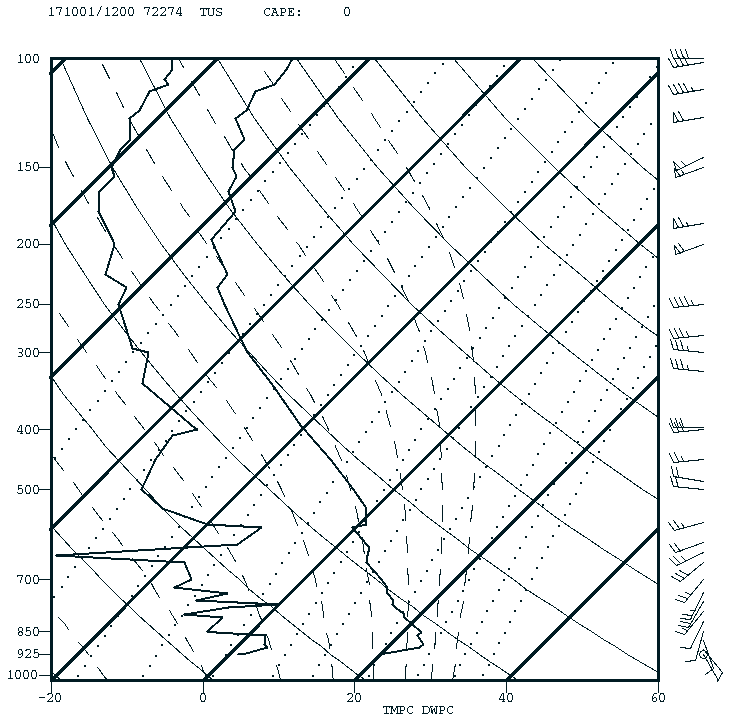
\includegraphics[width=\textwidth]{TUSTempProfile12Z.png}
  \caption{Temperature profile over Tucson, AZ on October 1, 2017 at 12Z (04:00 MST).}
  \label{fig:TUS12Z}
\end{figure}

\begin{enumerate}
  \item Looking at figures \ref{fig:TUS0Z} and \ref{fig:TUS12Z} it is hard to see any sharp abrupt changes in the lapse rate to signify the height of the tropopause, however, the lapse rare seems to slow down substantially near \SI{200}{\hecto\Pa} at 0Z and around \SIrange{225}{250}{\hecto\Pa} at 12Z.
  \item During the day at 0Z dry air appears to be neutral in the lower tropopause up until roughly \SI{650}{\hecto\Pa} indicating a rather large dry convective layer, above which it remains stable. At night (12Z), however, we see a temperature inversion near the surface indicating a highly unstable region up until \SI{850}{\hecto\Pa} above which it remains rather stable.
  \item During the day at 0Z (figure \ref{fig:TUS0Z}) we see the temperature profile follows an almost perfect dry adiabatic in the lower troposphere, while at night (12Z, figure \ref{fig:TUS12Z}) the surface cools and convection has moved the heat vertically upwards leading to a cooler surface with a warmer boundary layer right above it---a temperature inversion.
\end{enumerate}

\section{Dry convection case study}
Figure \ref{fig:YumaT} shows a temperature profile over Yuma, AZ while figure \ref{fig:YumaPotentialT} shows the corresponding potential temperature $\theta$ profile
\begin{equation*}
\theta(T,p) = T\left(\frac{p_0}{p}\right)^{R/c_p}
\end{equation*}
for approximate 2-hour intervals from 11:36 GMT to 21:39 GMT (04:36 to 14:39 MST) on a particular day. $R/c_p = 7/2$ for a dry atmosphere, as it is very closely approximated by an ideal diatomic gas with translation and rotational degrees of freedom, but not vibrational.

\begin{figure}[h!]
	\centering
	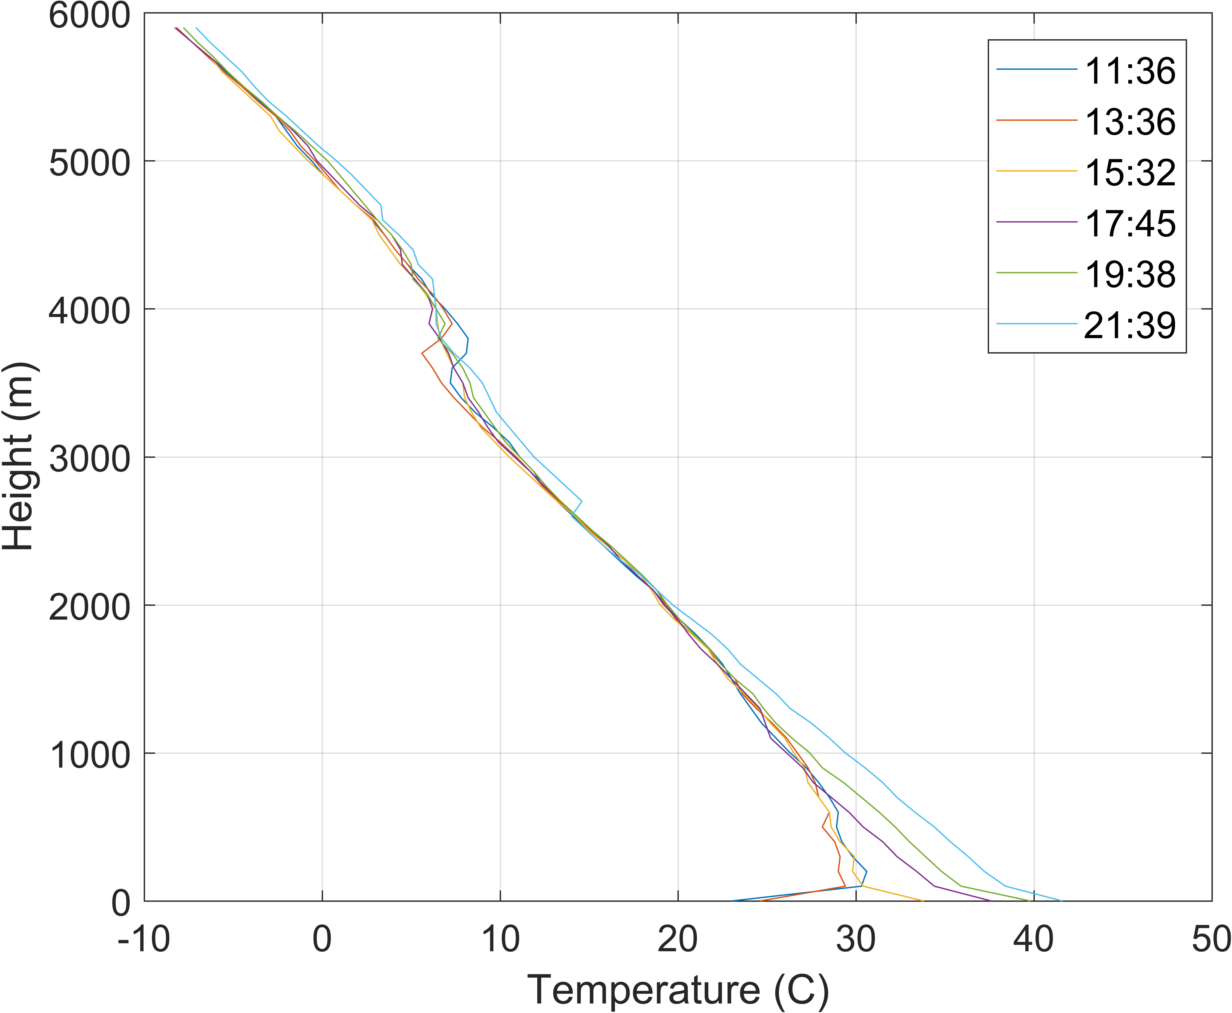
\includegraphics[width=\textwidth]{YumaTemp.png}
	\caption{Temperature profile over Yuma, AZ on a particular day from 11:36 GMT to 21:39 GMT (04:36 to 14:39 MST).}
	\label{fig:YumaT}
\end{figure}

\begin{figure}
	\centering
	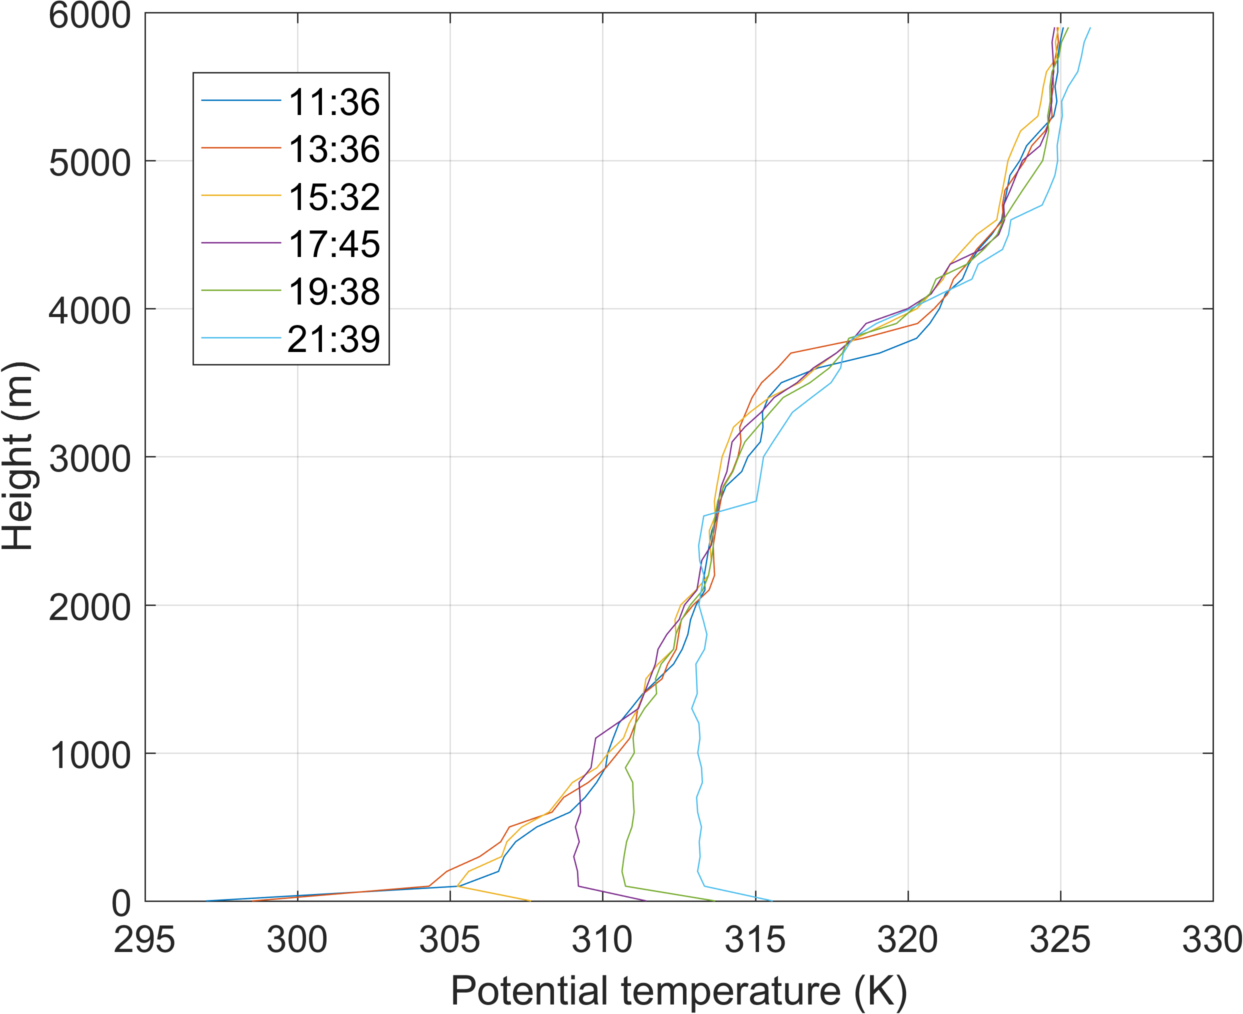
\includegraphics[width=\textwidth]{YumaPotentialTemp.png}
	\caption{Potential temperature profile over Yuma, AZ on a particular day from 11:36 GMT to 21:39 GMT (04:36 to 14:39 MST).}
	\label{fig:YumaPotentialT}
\end{figure}

Before the sun rises at 11:36 GMT and 13:36 GMT (03:36 and 05:36 MST), we notice a temperature inversion near the surface indicating that radiative cooling has taken place overnight leaving the surface cooler than the warmer air above it. For these two temperature profiles, dry air is highly unstable near the surface but then becomes rather neutral then stable past the first kilometer.

Once the sun is out at 15:32 GMT (07:32 MST) the surface begins to warm, undoing the temperature inversion that developed overnight. This trend continues throughout the day with the surface getting progressively warmer as indicated by the temperature profiles at 17:45, 19:38, and 21:39 GMT (9:45, 11:38, and 13:39 MST) until the dry air is neutrally buoyant all the way up to \SI{2}{\km}, indicating the presence of large dry convective cells. For these four profiles, we see that dry is still unstable in the lowest layer of the troposphere until it is well past noon with the 21:39 GMT (13:39 MST) profile, at which point the lowest layer is largely neutral.

\section{Moist convection}


%\begin{thebibliography}{9}
%\bibitem{AMSVirtualTemp}
%American Meteorological Society, cited 2012: Virtual temperature. Glossary of Meteorology. [Available online at \url{http://glossary.ametsoc.org/wiki/Virtual_temperature}]
%
%\bibitem{Wallace}
%Wallace, John M. and Peter V. Hobbs. \textit{Atmospheric Science; An Introductory Survey}. Elsevier. Second Edition, 2006. Chapter 1.
%\end{thebibliography}

\end{document}